\section{The Compact Muon Solenoid}\label{sec:cms}

The Compact Muon Solenoid is a hermetic detector and the smaller of the two multi-purpose experiments operating at the LHC at CERN.
The CMS detector covers the rapidity range $\eta < 3$ at full resolution and covers an extended range $\eta < 5$ with the bending power being provided by a 13m long, 6m inner diameter, 4T superconducting solenoid .
The need for such a magnet comes from the requirement to precisely measure the momentum of high-energy charged particles, for high momentum charged particles spend less time passing through magnetic fields, resulting in a less curved trajectory.
The more powerful the magnet, the more precisely high-energy charged particles can be measured due to their greater displacement\cite{oldcms}.

Moving away from the centre of the detector and the particle beam, CMS consists of the inner tracking system (a pixel tracker and a silicon microstrip tracker), an electromagnetic calorimeter (ECAL), a hadronic calorimeter (HCAL), a 4T superconducting solenoid, an outer calorimeter (HO), and the muon chambers.
There is also a pair of very-forward calorimeters (HF) in the extended rapidity region\cite{oldcms}.

The tracker, surrounding the interaction point, is designed to provide efficient precision trajectory measurements of charged particles emerging from collisions and precise reconstruction of secondary vertices over $\eta < 2.5$, whilst operating in a harsh radiation environment .
The tracker is composed of silicon, in order to limit charged particles interacting with the tracker (i.e. scattering, producing Bremsstrahlung), whilst providing the desired accuracy in track reconstruction\cite{oldcms}.

\begin{figure}[htbp]
\begin{center}
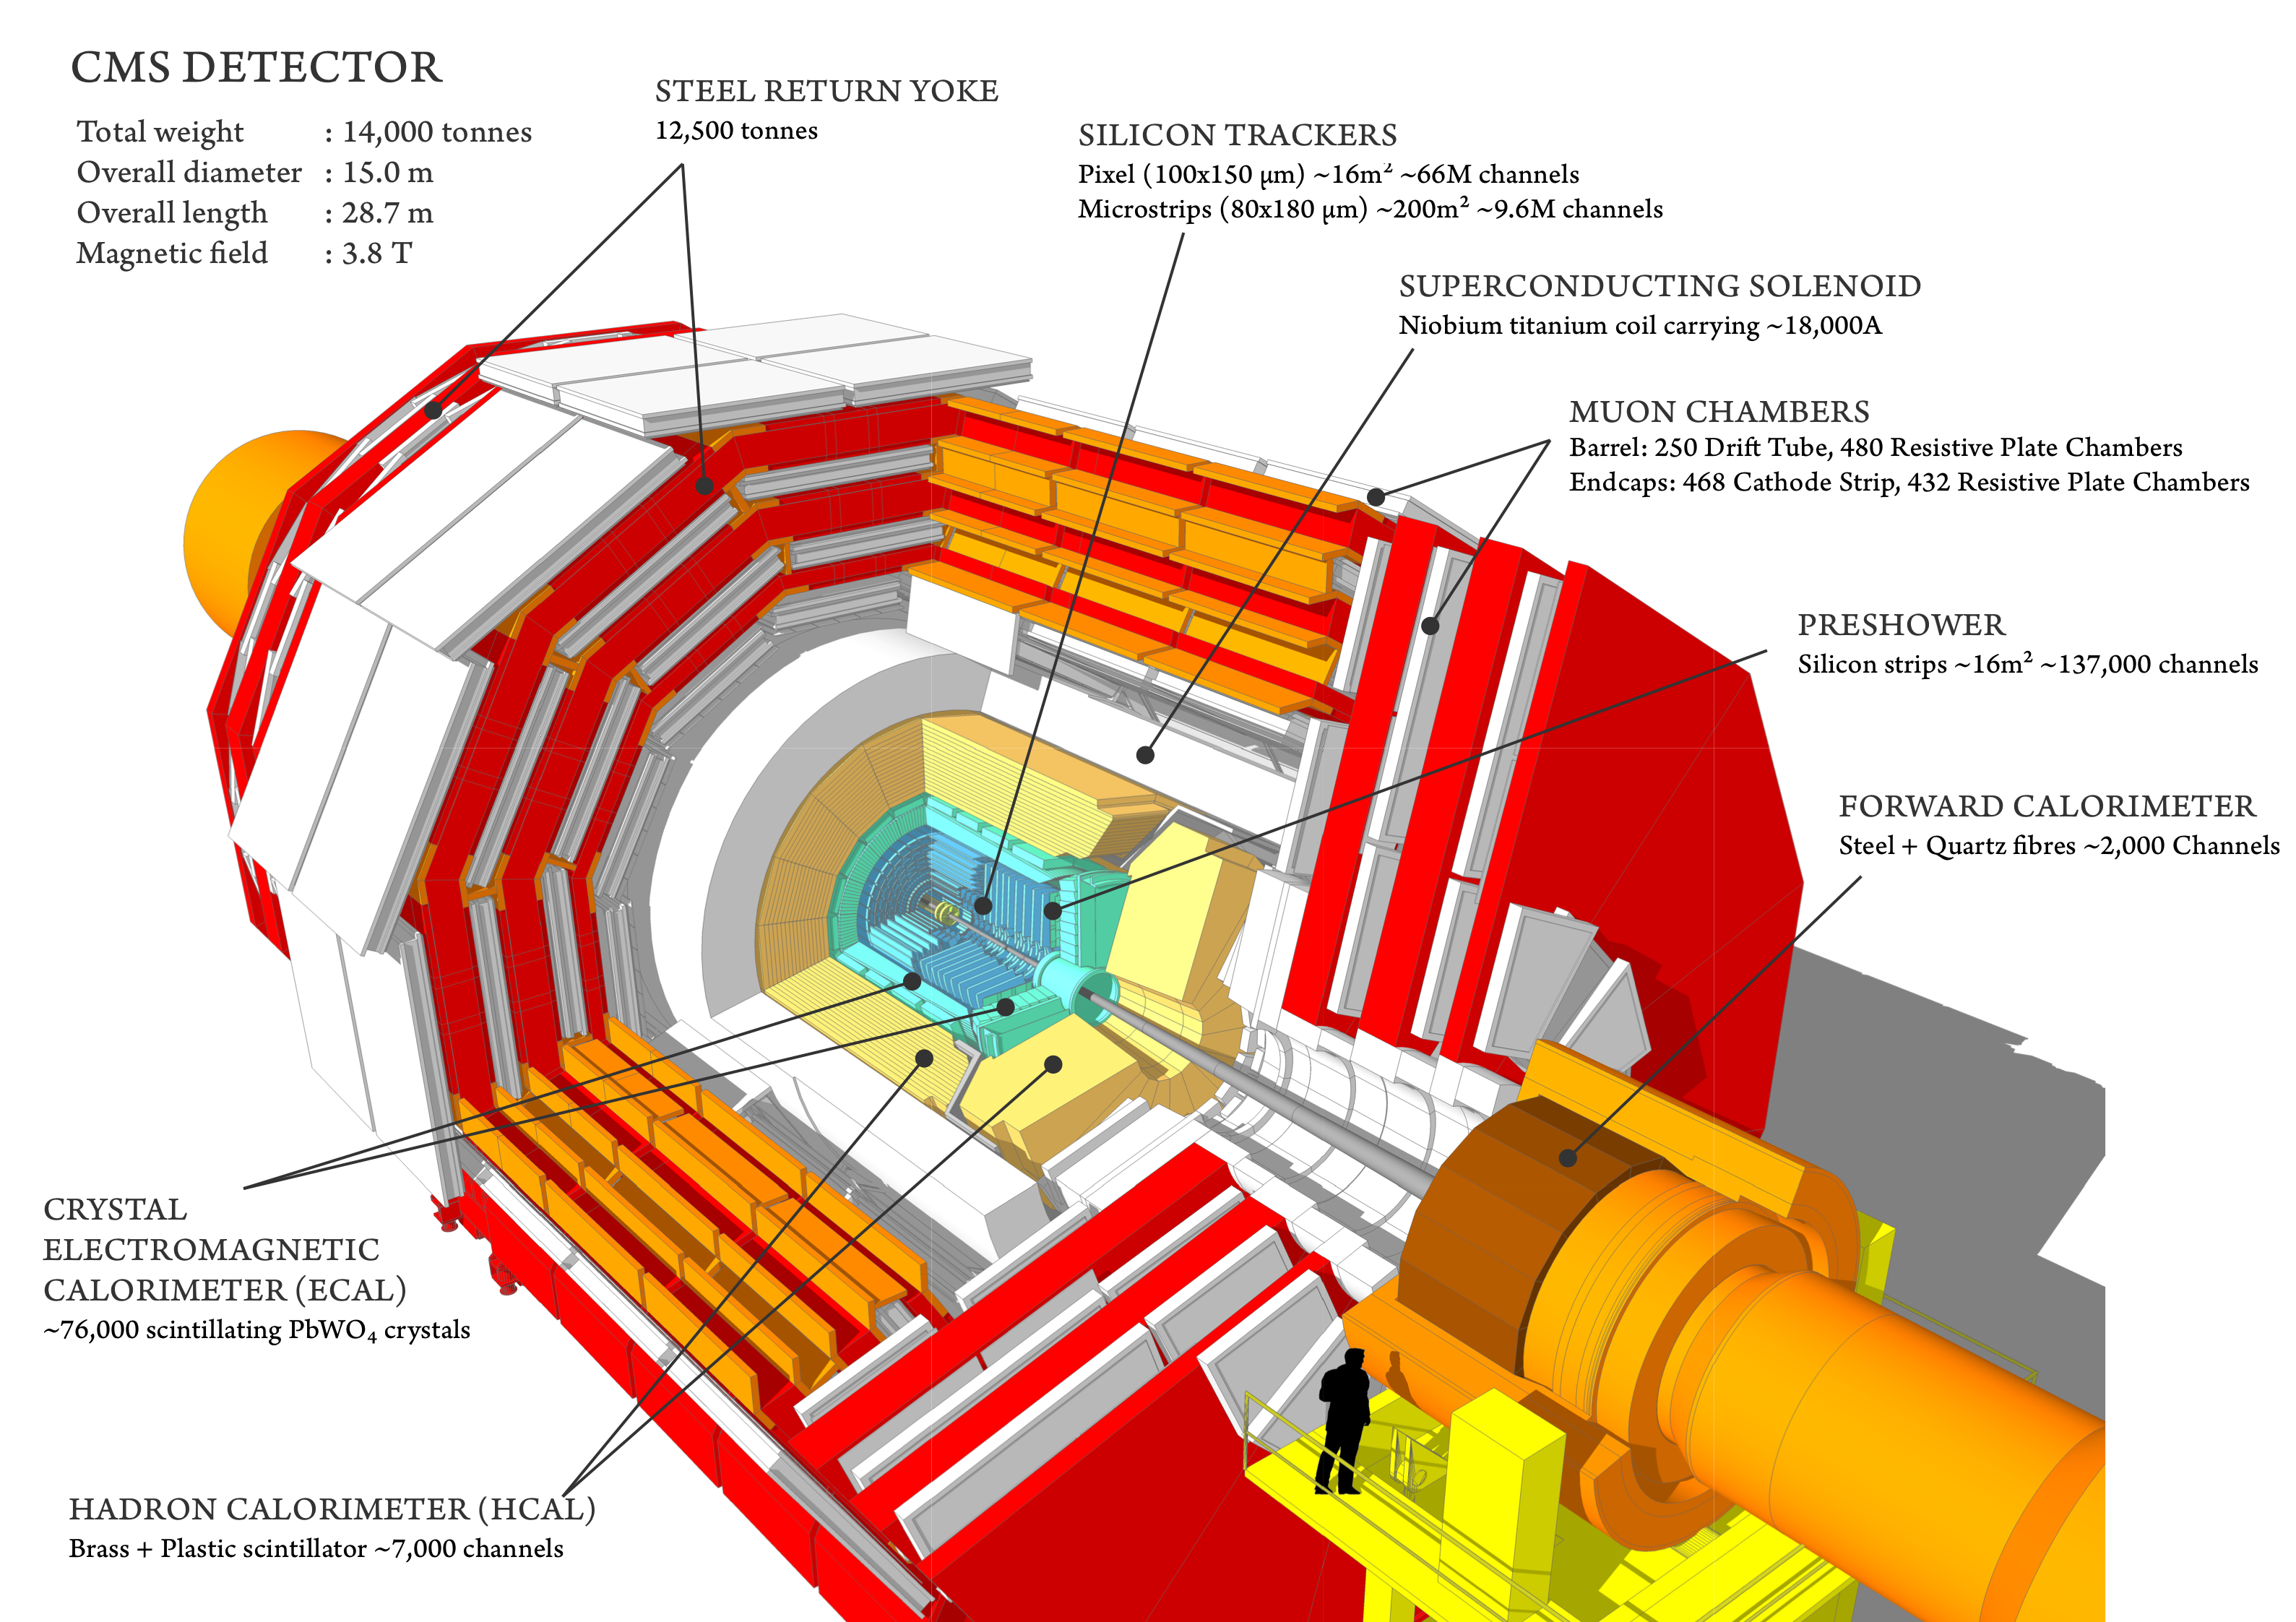
\includegraphics[width=0.97\textwidth]{figs/cms/cms_120918_03.png}
\caption{Cutaway diagram of CMS’s layers, illustrating its onion-like nature and the location of the detecting technologies within.}
\label{fig:cern-accelerator-complex}
\end{center}
\end{figure}

The ECAL measures the energies of electrons and fermions through the scintillations they cause, which are proportional to their energy, as they pass through it.
The very dense lead tungstate crystals only emit a small amount of light (which has to be amplified), the light they do emit is well defined, short, and fast, resulting in precise data with very little latency\cite{oldcms}. 

The HCAL, comprised of brass/steel absorber plates interspersed with plastic scintillators, measures hadrons energies over the barrel and endcap regions. 
There are also hadron calorimeters in the central rapidity region outside the solenoid coils (HO) and covering the extended $3.0 < \eta < 5.0$ rapidity region (HF)\cite{Bayatian:2006zz}. 

Detecting muons is incredibly important for CMS (as implied by the experiment’s name), given many of the signatures of interesting events involve them, including those from SUSY models and the so called “gold-plated” SM Higgs decay into a pair of Z0 bosons, which in turn decay into four muons . 
The gaseous muon detectors used are Drift Tubes (DTs), Cathode Strip Chambers (CSCs) and Resistive Plate Chambers (RPCs). 
The DTs and CSCs provide precise measurement coverage over the $\eta < 1.2$ (barrel) and $0.9 < \eta < 2.4$ (endcap) regions respectively. 
RPCs provide complimentary coverage over $\eta < 1.6$, and while having coarser position resolution than the DTs and CPCs, they have fast response times and excellent time resolution. 
Combining trigger candidates from the three systems gives an improved momentum resolution and efficiency than the stand-alone information from each of the individual systems\cite{oldcms}. 

\begin{figure}[htbp]
\begin{center}
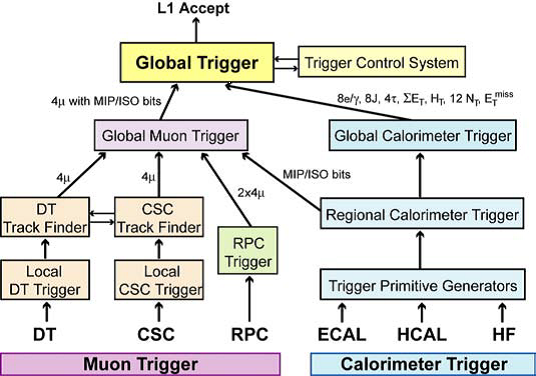
\includegraphics[width=0.97\textwidth]{figs/cms/trigger.png}
\caption{L-1 Trigger Architecture. Both muon and calorimeter triggers search for candidates locally before creating coarser datasets by passing on the most promising candidates to a higher level, and so on until the Global Trigger makes a final decision. However, unlike the Calorimeter Trigger, which looks at all the calorimeter systems concurrently, the Muon Trigger locally triggers on each of its detector technologies separately before submitting them to the Global Muon Trigger (with input from the Regional Calorimeter Trigger) before passing on fitted candidates to the Global Trigger.}
\label{fig:trigger}
\end{center}
\end{figure}

At design luminosity, there will be an event rate of $\sim$ 109 inelastic events/s . Given the impossibility of storing such a volume of data, let alone process it, the trigger system drastically reduces in two steps by selecting `interesting' events. 
The first step is the Level-1 (L1) Trigger, consisting of custom-designed programmable hardware (FPGA technology where possible). 
Initially both the calorimeter and muon triggers search over a small local area for the signature of an interesting event, forwarding these onto the regional triggers which sorts the candidates in order of importance, before the global calorimeter and muon triggers determine the highest ranked objects across the entire experiment. 
These are sent to the Global Trigger, which either rejects an event or accepts it for further evaluation by the second step, the High-Level-Trigger (HLT), a software system (see Fig.~\ref{fig:trigger} for a more detailed breakdown). 
Events accepted by the HLT are then transferred to mass storage for offline storage and analysis\cite{oldcms}. 

The L-1 trigger analyses every bunch crossing (BX). 
As such, there are strict time limitations on how long it takes for the data can be collected and read out. 
As the selection cannot be done before the subsequent BX, the current L-1 trigger uses a pipelined approach, providing a latency of $\approx$ 3.5\mus . 
Within the latency constraint for reducing the data rate, the L-1 trigger has to deal with the effects of the pileup of events, both in-time (within the same BX) and out-of-time (events from different BXs), in each BX . 
Additionally, the constraints on bandwidth limits the volume of data a single board can receive and determining whether events being read in. 
In light of this, the current approach of having large amounts of data over small regions being brought to fewer boards so that objects of interest can be considered, has to discard data at each stage a larger region is considered . 
While this approach creates candidates within these constraints, by definition only the candidates from this coarser data set can be considered. 
Any candidates in the discarded data are lost\cite{oldcms}.